\documentclass[12pt,a4paper]{article}
\usepackage[utf8]{inputenc}
\usepackage[margin=1in]{geometry}
\usepackage{graphicx}
\usepackage{float}
\usepackage{amsmath}
\usepackage{listings}
\usepackage{xcolor}

% Code listing style
\lstset{
    language=C++,
    basicstyle=\ttfamily\footnotesize,
    keywordstyle=\color{blue},
    commentstyle=\color{green},
    stringstyle=\color{red},
    numbers=left,
    numberstyle=\tiny,
    frame=single,
    breaklines=true
}

\begin{document}

% Front Page
\begin{titlepage}
  \centering
  \vspace*{3cm}

  {\Huge\bfseries CSE 406 – Lab Report 2: Shortest Job First (SJF) Non-Preemptive Scheduling Algorithm \par}
  \vspace{2.5cm}

  \noindent
  \begin{minipage}[t]{0.48\textwidth}
    {\large\bfseries Submitted By:}\\[0.5em]
    \Large
    Sharif Md. Yousuf \\
    ID: 22101128 \\
    Section: C-2 \\
    4th Year, 1st Semester \\
    Spring 2025
  \end{minipage}
  \hfill
  \begin{minipage}[t]{0.48\textwidth}
    {\large\bfseries Submitted To:}\\[0.5em]
    \Large
    Atia Rahman Orthi \\
    Lecturer \\
    Department of Computer Science \& Engineering \\
    University of Asia Pacific
  \end{minipage}

  \vfill

  {\Large\bfseries Date of Submission:} \\[0.5em]
  {\LARGE\bfseries 23 July, 2025 (Wednesday)}

  \vspace*{2cm}
\end{titlepage}

\section{Problem Statement}
An application is to be developed to perform the Shortest Job First-non-preemptive (SJF-NP) CPU scheduling. The name is a descriptive one in that it chooses a process, which has the smallest burst time amongst all processes that may be ready at a time, for execution. Processes may have diverse arrival times and can be scheduled only if they have arrived. Completion time, turnaround time, and waiting time are the minimum set of performance measures the code must give.

\section{Objective}
In this lab we:
\begin{itemize}
    \item Understood the operational principles of the SJF scheduling algorithm
    \item Implemented a non-preemptive version that selects jobs based on burst time
    \item Handled dynamic process arrivals and CPU idle time scenarios
    \item Calculated and analyzed scheduling performance metrics
    \item Compared the efficiency of SJF with other scheduling algorithms
\end{itemize}

\section{Source Code Screenshot}
\begin{figure}[H]
    \centering
    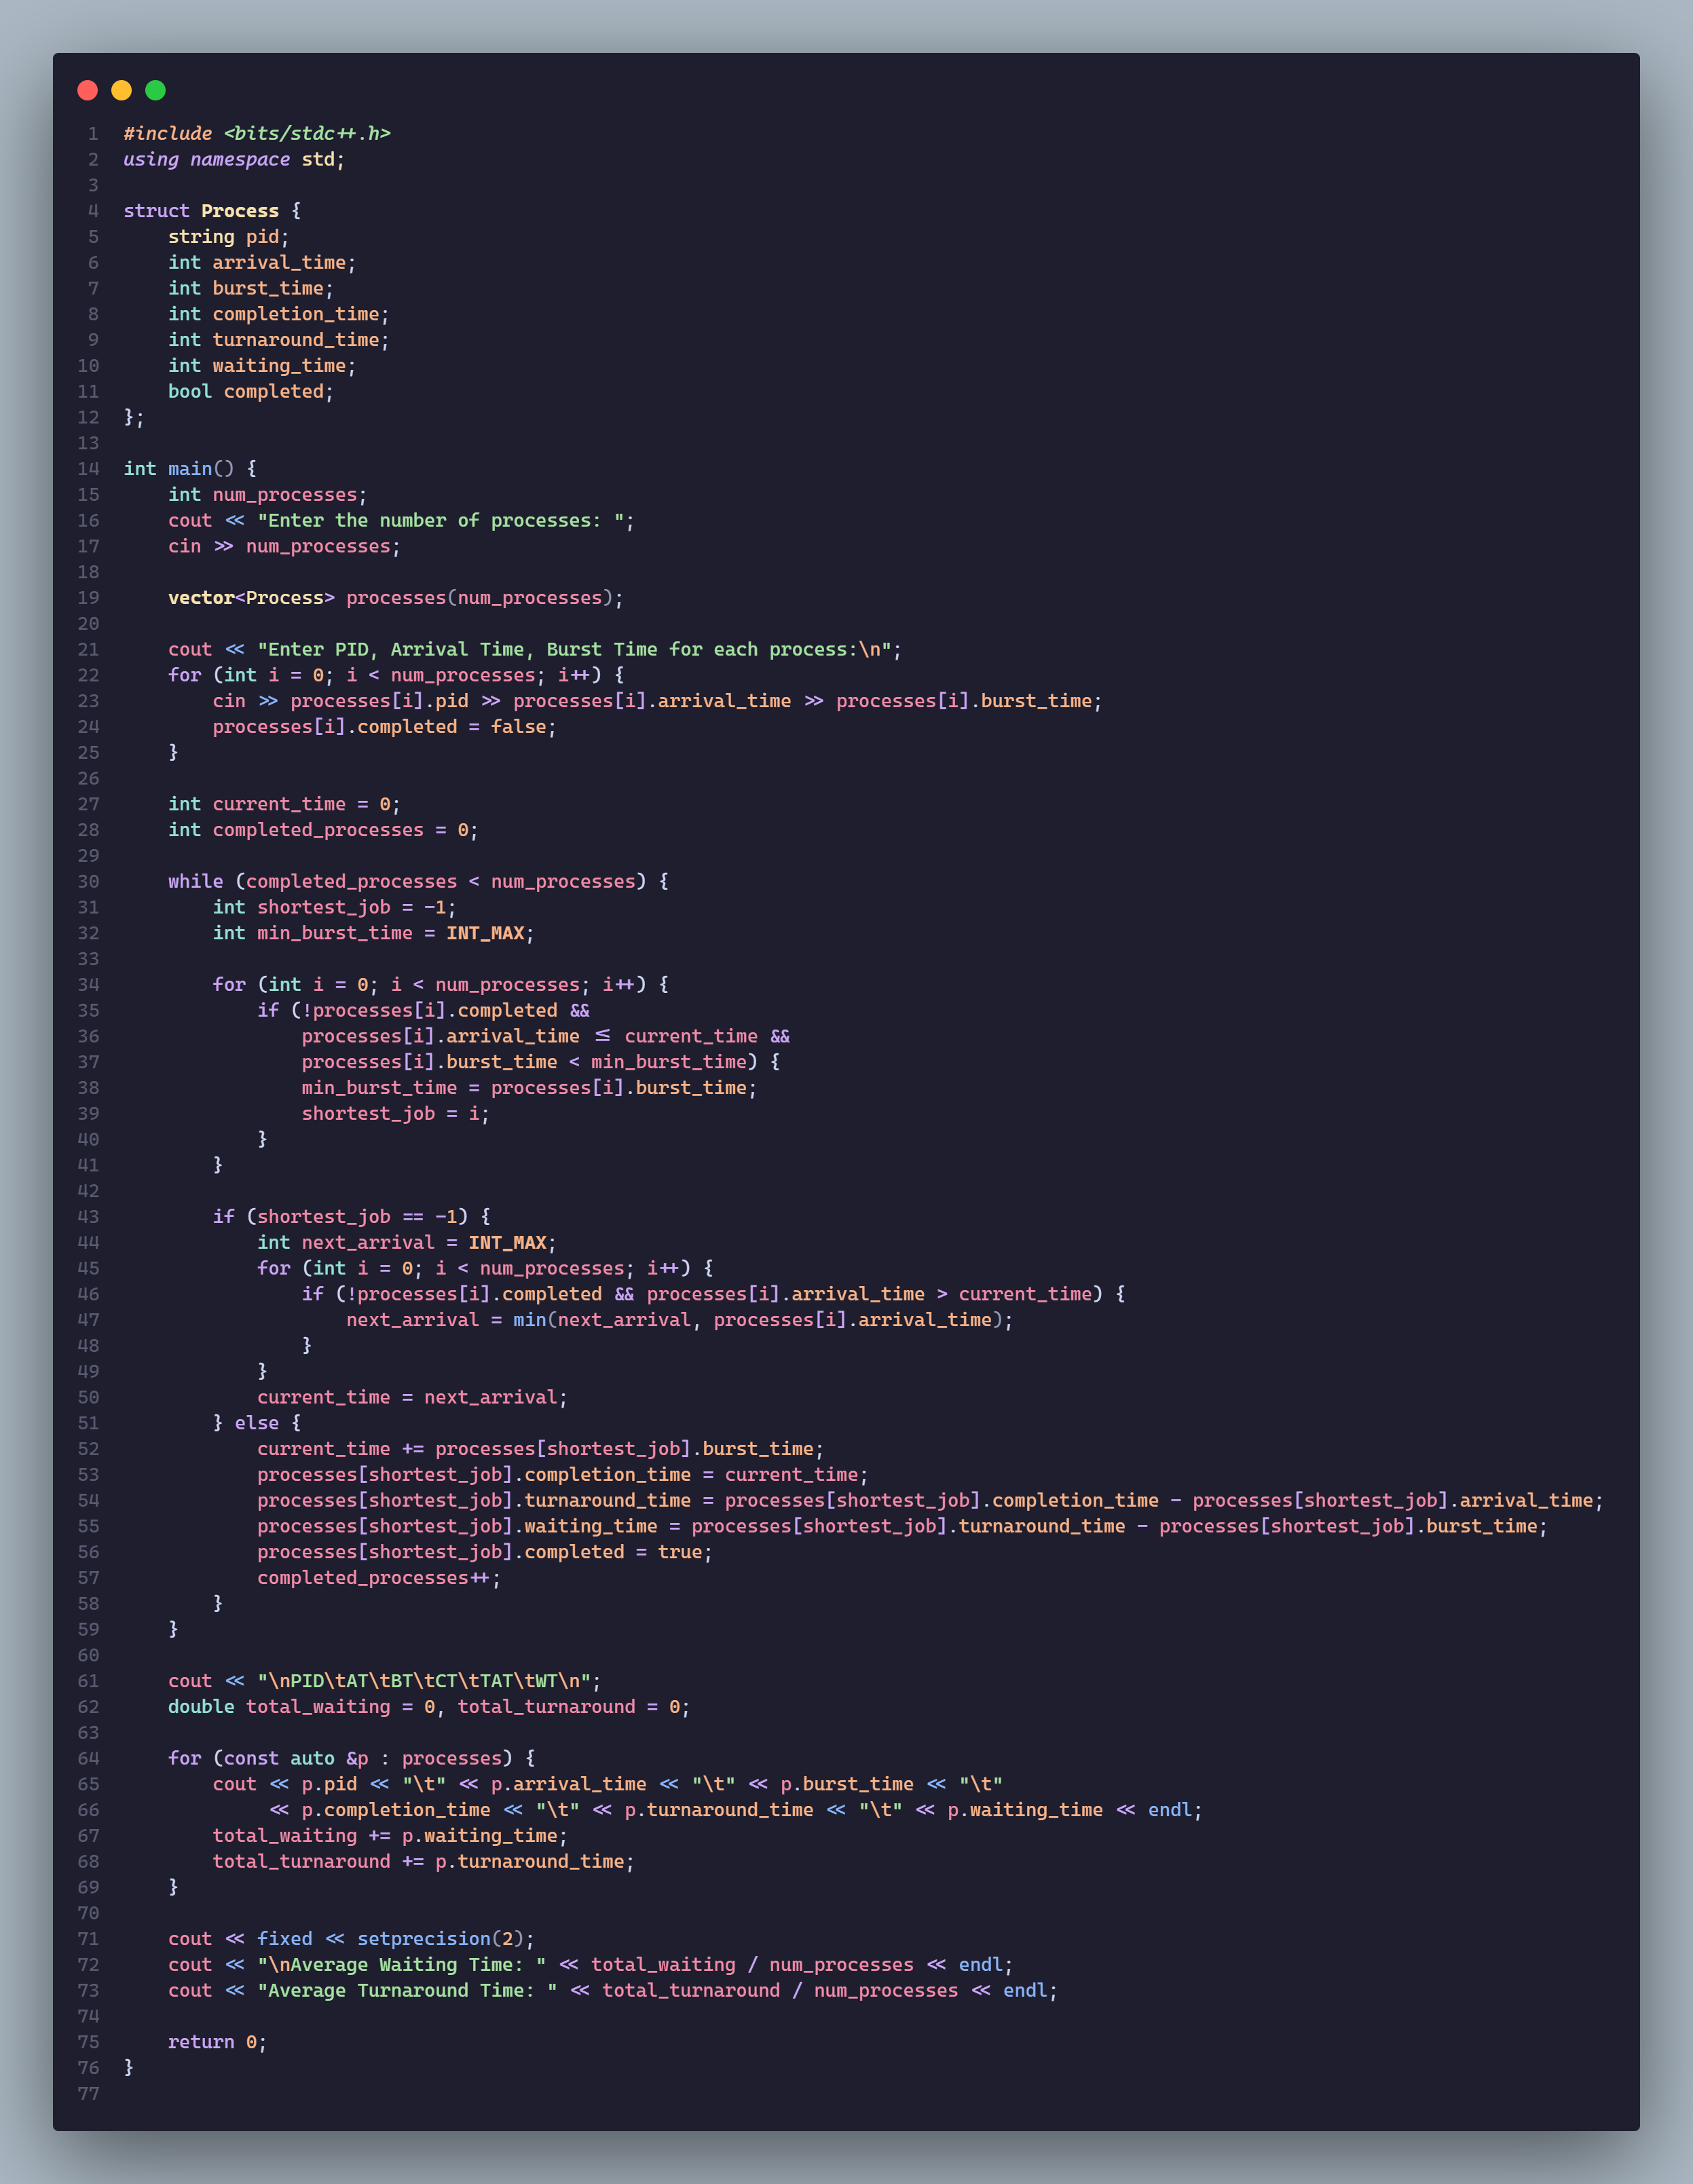
\includegraphics[width=0.8\textwidth]{code.png}
    \caption{SJF Non-Preemptive Algorithm Source Code}
    \label{fig:sjf_source}
\end{figure}

\section{Output Screenshot}
\begin{figure}[H]
    \centering
    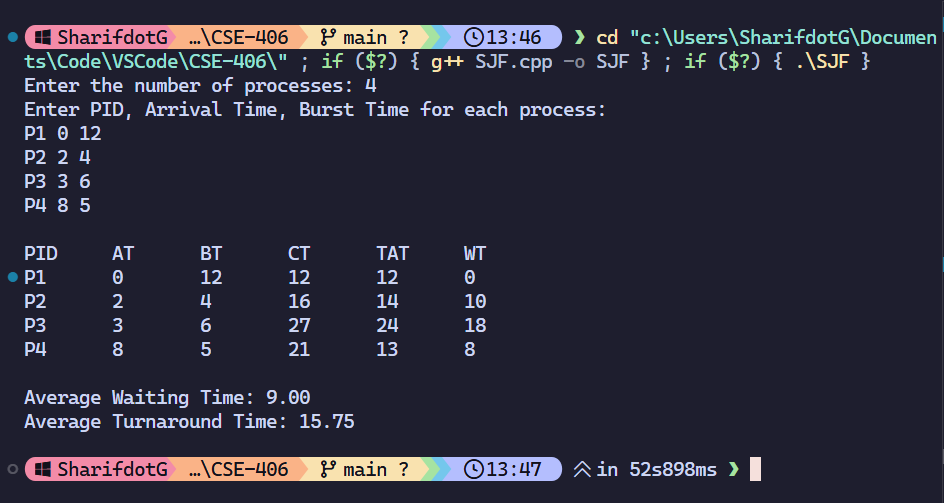
\includegraphics[width=0.8\textwidth]{Screenshot 2025-07-23 134801.png}
    \caption{SJF Algorithm Execution Output}
    \label{fig:sjf_output}
\end{figure}

\section{Discussion}
The SJF non-preemptive algorithm implementation provides an optimal solution for minimizing average waiting time among all non-preemptive scheduling algorithms. The algorithm operates by continuously selecting the process with the shortest burst time from the pool of arrived processes.

The implementation uses a while loop that continues until all processes are completed. At each iteration, it searches through all processes to find the one with the minimum burst time among those that have already arrived and are not yet completed. If no process is available (CPU idle situation), the algorithm advances the current time to the next process arrival time.

Important characteristics observed in this implementation:
\begin{itemize}
    \item The algorithm guarantees optimal average waiting time for non-preemptive schedulers
    \item It handles CPU idle time by jumping to the next arrival time when no processes are ready
    \item The selection process has O(n) complexity for each scheduling decision
    \item Starvation can occur if shorter processes keep arriving before longer ones complete
\end{itemize}

The algorithm effectively demonstrates the trade-off between optimality and complexity. While it provides better average performance than FCFS, it requires knowledge of burst times in advance, which is often not practical in real systems.

\section{Conclusion}
The SJF non-preemptive scheduling algorithm successfully minimizes average waiting time and provides optimal performance for batch processing systems where burst times are known. However, its practical implementation faces challenges due to the difficulty of predicting actual burst times. The algorithm works well in scenarios with predictable workloads but may cause starvation for longer processes. Despite these limitations, SJF serves as an important theoretical benchmark for comparing other scheduling algorithms and understanding the principles of optimal CPU scheduling.

\end{document}